%%%%%%%%%%%%%%%%%%%%%%%%%%%%%%%%%%%%%%%%%%%%%%%%%%%%%%%%%%%%%%%%%%%%%%%%%%%%%%%
%
% Filename: ira-analysis.tex
% Author:   David Oniani
% Modified: October 20, 2019
%  _         _____   __  __
% | |    __ |_   _|__\ \/ /
% | |   / _` || |/ _ \\  /
% | |__| (_| || |  __//  \
% |_____\__,_||_|\___/_/\_\
%
%%%%%%%%%%%%%%%%%%%%%%%%%%%%%%%%%%%%%%%%%%%%%%%%%%%%%%%%%%%%%%%%%%%%%%%%%%%%%%%

%%%%%%%%%%%%%%%%%%%%%%%%%%%%%%%%%%%%%%%%%%%%%%%%%%%%%%%%%%%%%%%%%%%%%%%%%%%%%%%
% Document definition
%%%%%%%%%%%%%%%%%%%%%%%%%%%%%%%%%%%%%%%%%%%%%%%%%%%%%%%%%%%%%%%%%%%%%%%%%%%%%%%

\documentclass[12pt]{article}

%%%%%%%%%%%%%%%%%%%%%%%%%%%%%%%%%%%%%%%%%%%%%%%%%%%%%%%%%%%%%%%%%%%%%%%%%%%%%%%
% Packages and related settings
%%%%%%%%%%%%%%%%%%%%%%%%%%%%%%%%%%%%%%%%%%%%%%%%%%%%%%%%%%%%%%%%%%%%%%%%%%%%%%%

% Global, document-wide settings
\usepackage[margin=1in]{geometry}
\usepackage[utf8]{inputenc}
\usepackage[english]{babel}

% Bibliography and references
\usepackage[backend=biber]{biblatex}
\addbibresource{$BIB}

% Math and alignment
\usepackage{multicol}
\usepackage{bookmark}
\usepackage{adjustbox}
\usepackage{braket}
\usepackage{mathtools}
\usepackage{amsmath}
\usepackage{amssymb}
\usepackage{amsthm}
\usepackage{amsfonts}
\usepackage{algorithmic}

% Graphics
\usepackage{pgfplots}
\pgfplotsset{compat=1.16}
\usepackage{tikz}
\usetikzlibrary{cd, arrows, decorations.markings}
\usepackage{graphicx}
\usepackage{rotating}
\usepackage{pst-solides3d}
\usepackage{xcolor}

% Fancy stuff
\usepackage{fancyhdr}
\usepackage{tocloft}
\usepackage{caption}
\usepackage{soul}
\usepackage{textcomp}
\usepackage{wasysym}
\usepackage[cache=false]{minted}
\usepackage{csquotes}
\usepackage{hyperref}
\usepackage{subfig}

%%%%%%%%%%%%%%%%%%%%%%%%%%%%%%%%%%%%%%%%%%%%%%%%%%%%%%%%%%%%%%%%%%%%%%%%%%%%%%%
% Mathematical operations and operators
%%%%%%%%%%%%%%%%%%%%%%%%%%%%%%%%%%%%%%%%%%%%%%%%%%%%%%%%%%%%%%%%%%%%%%%%%%%%%%%

% Sets and related operators
\newcommand{\nats}{\mathbb{N}}                   % Natural numbers
\newcommand{\pnats}{\mathbb{N}^+}                % Positive natural numbers

\newcommand{\ints}{\mathbb{Z}}                   % Integers
\newcommand{\pints}{\mathbb{Z}^+}                % Positive integers
\newcommand{\nints}{\mathbb{Z}^-}                % Negative integers

\newcommand{\rats}{\mathbb{Q}}                   % Rational numbers
\newcommand{\prats}{\mathbb{Q}^+}                % Positive rational numbers
\newcommand{\nrats}{\mathbb{Q}^-}                % Negative rational numbers

\newcommand{\reals}{\mathbb{R}}                  % Real numbers
\newcommand{\preals}{\mathbb{R}^+}               % Positive real numbers
\newcommand{\nreals}{\mathbb{R}^-}               % Negative real numbers

\newcommand{\irrats}{\mathbb{I}}                 % Irrational numbers

\newcommand{\pset}{\mathcal{P}}                  % Powerset
\newcommand{\card}{\abs}                         % Cardinality
\newcommand{\topology}{\mathcal{T}}              % Topology
\newcommand{\basis}{\mathcal{B}}                 % Basis
\newcommand{\oldemptyset}{\emptyset}             % Old empty set
\renewcommand{\emptyset}{\varnothing}            % New and nice empty set

% Other operators
\DeclarePairedDelimiter\abs{\lvert}{\rvert}      % Absolute value
\DeclarePairedDelimiter\ceil{\lceil}{\rceil}     % Ceiling
\DeclarePairedDelimiter\floor{\lfloor}{\rfloor}  % Floor

%%%%%%%%%%%%%%%%%%%%%%%%%%%%%%%%%%%%%%%%%%%%%%%%%%%%%%%%%%%%%%%%%%%%%%%%%%%%%%%
% Command definitions and redefinitions
%%%%%%%%%%%%%%%%%%%%%%%%%%%%%%%%%%%%%%%%%%%%%%%%%%%%%%%%%%%%%%%%%%%%%%%%%%%%%%%

% New commands
\newcommand{\rarr}{\rightarrow}                        % Leftarrow
\newcommand{\larr}{\leftarrow}                         % Rightarrow
\newcommand\und[1]{\underline{\smash{#1}}}             % Nice-looking underline

% Renewed commands
\renewcommand{\headrulewidth}{0.5pt}                   % Header rule width
\renewcommand{\footrulewidth}{0pt}                     % Footer rule width
\renewcommand{\baselinestretch}{1.5}                   % Line spacing is 1.5
\renewcommand{\cftsecleader}{\cftdotfill{\cftdotsep}}  % Dots for ToC sections

% Rename "Contents" to "Table of Contents"
\addto\captionsenglish{% Replace "english" with the language used
  \renewcommand{\contentsname}%
    {\textbf{Table of Contents}}}%

% Filling the space for centering the title of the table of contents
\renewcommand{\cfttoctitlefont}{\hspace*{\fill}\Large}
\renewcommand{\cftaftertoctitle}{\hspace*{\fill}}

%%%%%%%%%%%%%%%%%%%%%%%%%%%%%%%%%%%%%%%%%%%%%%%%%%%%%%%%%%%%%%%%%%%%%%%%%%%%%%%
% Miscellaneous
%%%%%%%%%%%%%%%%%%%%%%%%%%%%%%%%%%%%%%%%%%%%%%%%%%%%%%%%%%%%%%%%%%%%%%%%%%%%%%%

% Setting stuff
\setlength{\parindent}{0pt}  % Remove indentations from paragraphs
\frenchspacing               % Get rid of large spaces after dots
\pagestyle{fancy}            % This allows to do fancy headers and footers
\fancyhf{}                   % No additional page numbering (or other stuff)
\cfoot{\thepage}             % Display page number at the bottom, in the center

% PDF information and nice-looking urls
\hypersetup{%
  pdfauthor  = {David Oniani},
  pdftitle   = {Textual and Statistical Analysis of Russian IRA Facebook Posts},
  pdfsubject = {Statistics, Authorship Attribution, Visual Persuasion},
  colorlinks = true,
  linkcolor  = {blue!50!black},
  citecolor  = {blue!50!black},
  urlcolor   = {blue!50!black}
}

% Put a centered header of a footnote size on the top of each page
\chead{\footnotesize{\MakeUppercase{Textual and Statistical Analysis of Russian IRA Facebook Posts}}}

% Definition environment
\theoremstyle{definition}
\newtheorem*{definition}{Definition}

%%%%%%%%%%%%%%%%%%%%%%%%%%%%%%%%%%%%%%%%%%%%%%%%%%%%%%%%%%%%%%%%%%%%%%%%%%%%%%%
% Author(s), title, and date
%%%%%%%%%%%%%%%%%%%%%%%%%%%%%%%%%%%%%%%%%%%%%%%%%%%%%%%%%%%%%%%%%%%%%%%%%%%%%%%

% Author(s)
\author{David Oniani\\
        Luther College\\
        \href{mailto:oniada01@luther.edu}{oniada01@luther.edu}}

% Title
\title{\textbf{Textual and Statistical Analysis of Russian IRA Facebook Posts}\\
      \small \textsuperscript{*}The paper is written in the scope of a student-faculty collaborative\\
                                summer research with professor Richard K. Merritt (\href{mailto:merritri@luther.edu}{merritri@luther.edu}).}

% Date
\date{October 25, 2019}

%%%%%%%%%%%%%%%%%%%%%%%%%%%%%%%%%%%%%%%%%%%%%%%%%%%%%%%%%%%%%%%%%%%%%%%%%%%%%%%
% Beginning of the document
%%%%%%%%%%%%%%%%%%%%%%%%%%%%%%%%%%%%%%%%%%%%%%%%%%%%%%%%%%%%%%%%%%%%%%%%%%%%%%%

\begin{document}
\maketitle

%%%%%%%%%%%%%%%%%%%%%%%%%%%%%%%%%%%%%%%%%%%%%%%%%%%%%%%%%%%%%%%%%%%%%%%%%%%%%%%
% Abstract
%%%%%%%%%%%%%%%%%%%%%%%%%%%%%%%%%%%%%%%%%%%%%%%%%%%%%%%%%%%%%%%%%%%%%%%%%%%%%%%

\begin{abstract}
\addcontentsline{toc}{section}{Abstract}

\noindent The 2016 United States Presidential Election was targeted by an
unprecedented intelligence and influence campaign. Arising out of Russian
so-called Internet Research Agency (IRA), it sought to sow discord, attack
the fissures of the United States, and ultimately, sway the election results.
~\cite{ira2016}~\cite{ira2016data} Recently, some of the IRA-backed Facebook
advertisements were released by The United States House Permanent Select
Committee on Intelligence. All of the advertisements are in the PDF format. We
have scraped the PDF files and present the results obtained by both textual and
statistical analyses of the above-mentioned data. Authorship attribution and
sentiment analysis were also performed.~\footnote{Please note that this paper
does not discuss the political implications of these actions, but attempts to
explore the methods of persuasion that were employed in this influence
campaign.}~\cite{ira2016csvdata} In addition, we have made the data publicly
available for other researchers and/or interested people in a much nicer and
easier-to-manipulate CSV format.
\end{abstract}

%%%%%%%%%%%%%%%%%%%%%%%%%%%%%%%%%%%%%%%%%%%%%%%%%%%%%%%%%%%%%%%%%%%%%%%%%%%%%%%
% Table of Contents
%%%%%%%%%%%%%%%%%%%%%%%%%%%%%%%%%%%%%%%%%%%%%%%%%%%%%%%%%%%%%%%%%%%%%%%%%%%%%%%

\newpage
\tableofcontents
\newpage

%%%%%%%%%%%%%%%%%%%%%%%%%%%%%%%%%%%%%%%%%%%%%%%%%%%%%%%%%%%%%%%%%%%%%%%%%%%%%%%
% Data and Preparation
%%%%%%%%%%%%%%%%%%%%%%%%%%%%%%%%%%%%%%%%%%%%%%%%%%%%%%%%%%%%%%%%%%%%%%%%%%%%%%%

\section*{\centering Data and Preparation}
\addcontentsline{toc}{section}{Data and Preparation}

The dataset was scraped from~\cite{ira2016data} more than 3,500 Russian IRA
Facebook posts made publicly available in the PDF format by the House
Intelligence Committee. We used the free and open-source Python library
~\cite{pdftotext} \texttt{pdftotext} to scrape the data. Many CSV files were
formatted in a way that it was virtually impossible for \texttt{pdftotext} to
parse them correctly. Due to this reason, we have manually reviewed most of the
CSV files for validity.~\cite{ira2016csvdata} All the CSV files have been made
publicly available. It is important to note that the dataset is just a sample
of a bigger dataset and, albeit \textit{less likely}, might not be a good
representatation of the overall campaign.

%%%%%%%%%%%%%%%%%%%%%%%%%%%%%%%%%%%%%%%%%%%%%%%%%%%%%%%%%%%%%%%%%%%%%%%%%%%%%%%
% Common Words
%%%%%%%%%%%%%%%%%%%%%%%%%%%%%%%%%%%%%%%%%%%%%%%%%%%%%%%%%%%%%%%%%%%%%%%%%%%%%%%

\section*{\centering Common Words}
\addcontentsline{toc}{section}{Common Words}

Among the strategies utilized by this influence campaign, one that stood out
the most was the exploitation of internal issues of the United States by
realizing social, political, and historical backgrounds of the country.
This was achieved primarily by using words and phrases strongly linked to the
above-mentioned issues.

\bigskip

The words choice played a crucial role in the persuasive quality of posts.
Below is the barchart showing top 25 most commonly used words after eliminating
linking verbs, prepositions, pronouns, and some other
~\footnote{The list of all eliminated words is provided at\\
\url{https://github.com/oniani/ira-analysis/blob/master/eliminated-words.txt}.}
non-relevant words. Three most commonly used words in the campaign were black,
police, and people.

\begin{figure}[H]
\centering
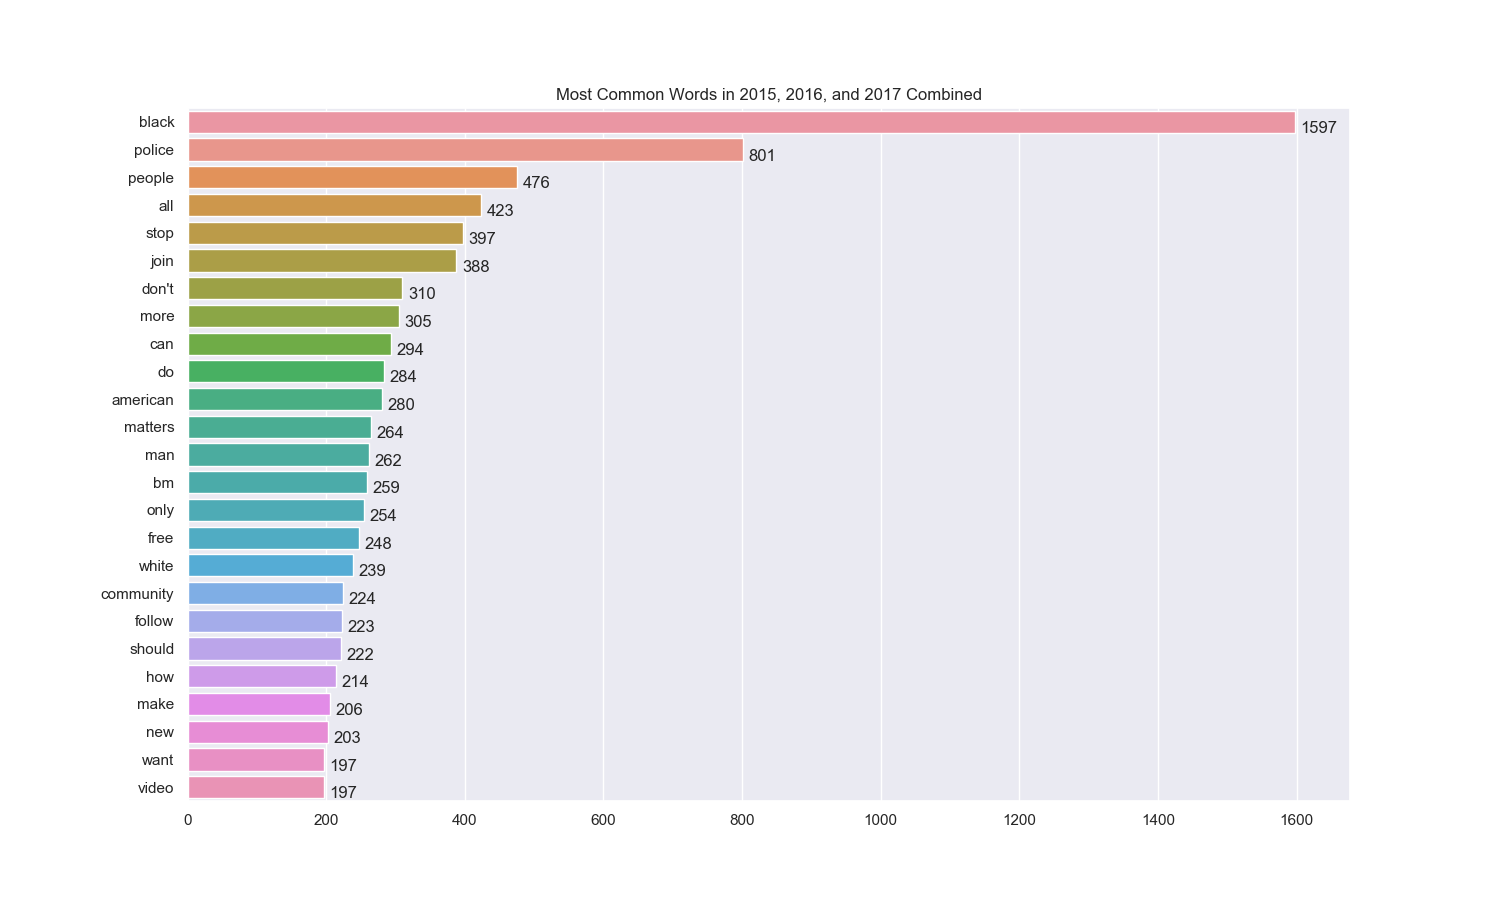
\includegraphics[width=\columnwidth]{./image/barchart-plots/barchart_word_counts.png}
\caption{Most common words in 2015, 2016, and 2017 combined.}
\end{figure}

It is apparent that the vast majority of the Facebook posts featured words and
phrases related to race and race-based discrimination. Words related to
``taking action'' such as ``join'', ``stop'', ``do'', ``follow'' etc. were used
extensively for persuasive purposes. These words in combination with other words
like ``american'', ``matters'', ``community'' etc.~further increased the
persuasive quality of the advertisement by metaphorically connecting it with
cultural and social identities of people.

%%%%%%%%%%%%%%%%%%%%%%%%%%%%%%%%%%%%%%%%%%%%%%%%%%%%%%%%%%%%%%%%%%%%%%%%%%%%%%%
% Sentiment Analysis
%%%%%%%%%%%%%%%%%%%%%%%%%%%%%%%%%%%%%%%%%%%%%%%%%%%%%%%%%%%%%%%%%%%%%%%%%%%%%%%

\section*{\centering Sentiment Analysis}
\addcontentsline{toc}{section}{Sentiment Analysis}

For the sentiment analysis purposes, we used \texttt{python}'s
\texttt{TextBlob} library. Suprisingly, out of all Facebook posts with
non-empty \texttt{Ad Text} value, 1643 were positive, 900 negative, and 933
neutral leaving the overall tone of the posts positive. Yet, the statistical
significance of this claim is rather questionable as the polarity levels were
always near zero. Such low polarity level, however, demonstrates a highly
intelligent design of advertisements.

\bigskip

As the \texttt{Ad Text}s did not give us any strong evidences, we looked at the
negativity levels across all three years and found a consistent trend (Figure 2).

\begin{figure}[H]
\centering
\begin{tabular}{|p{3cm}|p{3cm}|p{3cm}|p{3cm}|p{3cm}|}
 \hline
 Subjectivity & Year 2015 & Year 2016 & Year 2017 & 2016 (\%)\\
 \hline
 1.0  & 154 & 562 & 176 & 63.004\\
 \hline
 0.75 & 150 & 547 & 169 & 63.164\\
 \hline
 0.5  & 123 & 405 & 120 & 62.500\\
 \hline
 0.25 & 15  & 81  & 22  & 68.644\\
 \hline
 0.15 & 5   & 33  & 10  & 68.750\\
 \hline
 0.1  & 2   & 11  & 6   & 57.895\\
 \hline
 0.05 & 1   & 5   & 2   & 62.500\\
 \hline
\end{tabular}
\caption{Analyzing Negativity}
\end{figure}

\bigskip

Notice that for any given year and at any subjectivity level, year 2016 is
consistently comprising around 60\% of all posts. The suddent change in
strategy and increased levels of negativity could be linked to making people
take an action by voting for candidates promoted by these ads. The year of the
Presidential Election was rather negative.

%%%%%%%%%%%%%%%%%%%%%%%%%%%%%%%%%%%%%%%%%%%%%%%%%%%%%%%%%%%%%%%%%%%%%%%%%%%%%%%
% Authorship Attribution
%%%%%%%%%%%%%%%%%%%%%%%%%%%%%%%%%%%%%%%%%%%%%%%%%%%%%%%%%%%%%%%%%%%%%%%%%%%%%%%

\section*{\centering Authorship Attribution}
\addcontentsline{toc}{section}{Authorship Attribution}

Since all of these posts were issued by the same organization/entity, it was
interesting to see if there are some common patterns between the Facebook ads
of 2015, 2016, 2017. For this reason, we have performed authorship attribution
tests by implementing~\cite{koppel11} the paper by Koppel et.~al.

\bigskip

We have performed 3 authorship attribution tests:

\begin{enumerate}
  \item Assuming that the author of the Facebook posts of 2016 and 2017 was the
        same and checking accuracy for the author of 2015.

  \item Assuming that the author of the Facebook posts of 2015 and 2017 was the
        same and checking accuracy for the author of 2016.

  \item Assuming that the author of the Facebook posts of 2015 and 2016 was the
        same and checking accuracy for the author of 2017.
\end{enumerate}

In all three cases, we had to merge different posts to meet the required
minimum text length of 500 words.~\footnote{Note that because of randomization,
texts were somewhat scrambled and are not available in any format. That said,
one can easily redo the authorship attribution with similar accuracy using the
algorithm which is already implemented and resides in the GitHub repository,
\url{https://github.com/oniani/ira-analysis/tree/master/koppel11}.} This was
done using randomization to avoid bias.~\footnote{Results JSON:
\url{https://github.com/oniani/ira-analysis/tree/master/koppel11/results}}
Results are available in the form of JSON files formatted in the manner shown
below.

\begin{figure}[H]
\begin{minted}[frame=single, linenos=true, tabsize=2]{js}
{
  "answers": [
    {
      "unknown_text": "2015-unknown1.txt",
      "author": "candidate2016",
      "score": 0.58
    },
    ...
    {
      "unknown_text": "2015-unknown56.txt",
      "author": "candidate2016",
      "score": 0.76
    }
  ]
}
\end{minted}
\caption{JSON example}
\end{figure}

The first answer tells us that the unknown text was written in year 2015, and
that there is 58\% chance that it was written by the author of Facebook posts
of 2016. The last answer shows that there is 0.76\% chance that the given
text was authored by the entity who wrote the posts in year 2016.

\bigskip

Figure 4 shows the results obtained after performing all three above-mentioned
authorship attribution tests.

\begin{figure}[H]
\centering
\begin{tabular}{|p{8cm}|p{8cm}|}
 \hline
 Years & Similarity (\%)\\
 \hline
 2016 and 2017 & 72.509 (similarity to 2015)\\
 \hline
 2015 and 2017 & 68.516 (similarity to 2016)\\
 \hline
 2015 and 2016 & 62.392 (similarity to 2017)\\
 \hline
 Average (2015, 2016, and 2017) & 67.806\%\\
 \hline
\end{tabular}
\caption{Average Similarity}
\end{figure}

On average, there is approximately 68\% similarity across texts suggesting that
the design strategy for these posts were roughly similar.

%%%%%%%%%%%%%%%%%%%%%%%%%%%%%%%%%%%%%%%%%%%%%%%%%%%%%%%%%%%%%%%%%%%%%%%%%%%%%%%
% General Statistics
%%%%%%%%%%%%%%%%%%%%%%%%%%%%%%%%%%%%%%%%%%%%%%%%%%%%%%%%%%%%%%%%%%%%%%%%%%%%%%%

\section*{\centering General Statistics}
\addcontentsline{toc}{section}{General Statistics}

The distribution of posts over all three years shows a bimodal nature with two
peaks in quarters 2 and 4 of year 2016. Given the fact that the US Presidential
Election was held in the fourth quarter of 2016, it is surprising that the
number of posts in the second quarter exceeded that of the fourth quarter.

\begin{figure}[H]
\centering
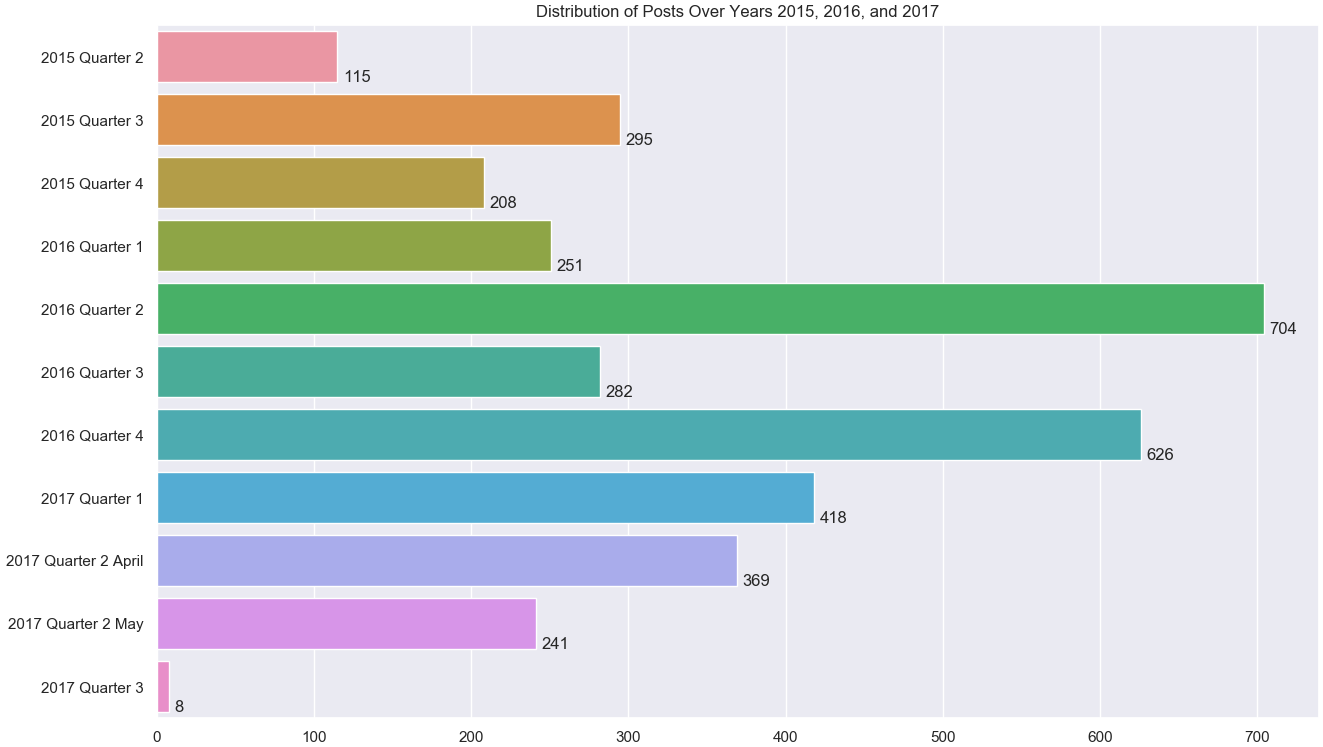
\includegraphics[width=\columnwidth]{./image/barchart-plots/barchart_distribution_of_posts.png}
\caption{Distribution of Posts Over Years 2015, 2016, and 2017.}
\end{figure}

As for the ad spendings, the fourth quarter of 2016 exceeds that of any quarter,
with second quarter coming next. Interestingly, most of ads were paid in the
Russian currency (ruble) with two exceptions (4 posts in total) in 2016 quarter
3 and 2017 quarter 1 when IRA spent \$74.000 and \$35.330 respectively.

\begin{figure}[H]
\centering
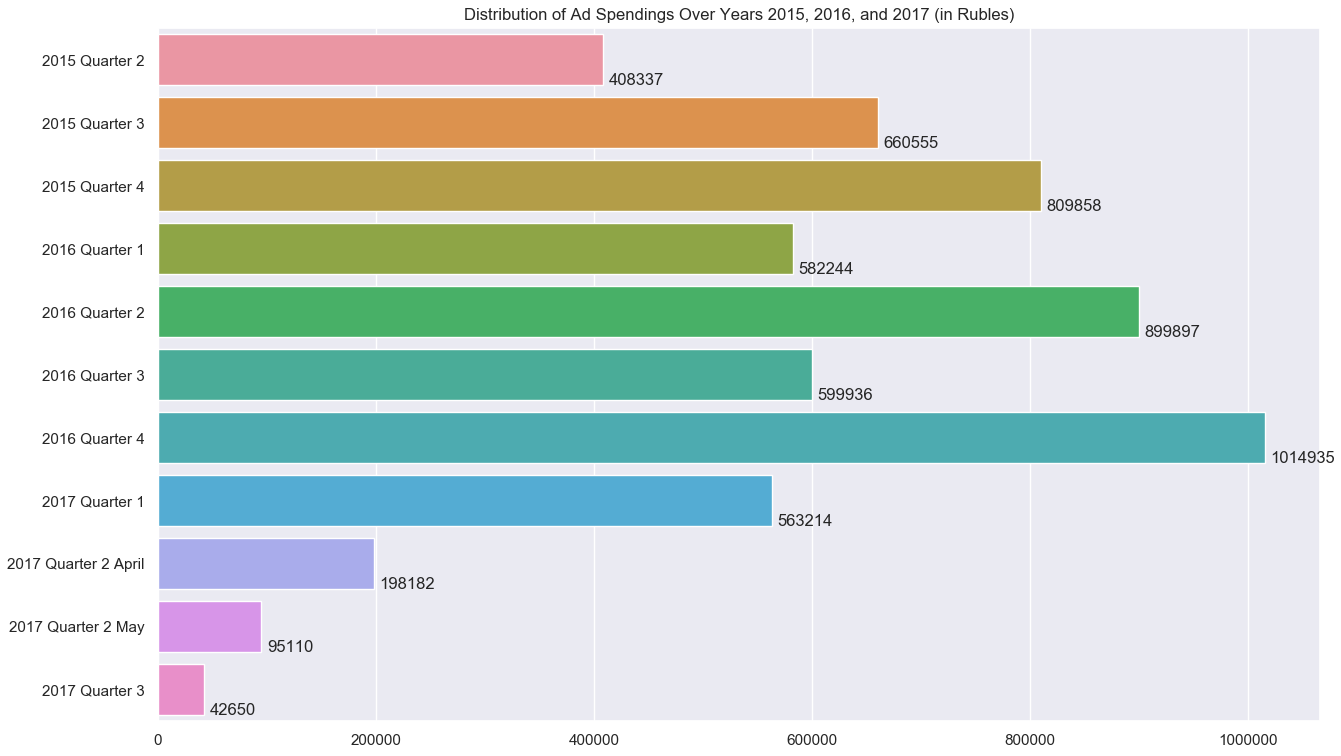
\includegraphics[width=\columnwidth]{./image/barchart-plots/barchart_ad_spend_RU_distribution.png}
\caption{Distribution of Ad Spendings Over Years 2015, 2016, and 2017 (in rubles).}
\end{figure}

Furthermore, 99.8\% of all paid ads across all years were paid in rubles.
Figure 7 shows a chart with the number of posts based on a currency.

\begin{figure}[H]
\begin{center}
\begin{tabular}{|p{3cm}|p{3cm}|}
 \hline
 Currency & \text{Total (All Years)}\\
 \hline
 RUB  & 2549\\
 \hline
 USD  & 5\\
 \hline
 ~\footnote{None values can be considered 0} None & 787\\
 \hline
 0    & 176\\
 \hline
\end{tabular}
\end{center}
\caption{Number of Posts Depending on the Currency.}
\end{figure}

\bigskip

As the information for the reader, the Russian ruble is used only in Russia,
Belarus, and two regions of Georgia, which are considered by Russia as partially
recognized states of Abkhazia and South Ossetia.

IRA was rather liberal toward age with 69.542\% of all advertisements being
targeted toward individuals aging from 18 up. Figure 8 shows the distribution
of these ads.

\begin{figure}[H]
\centering
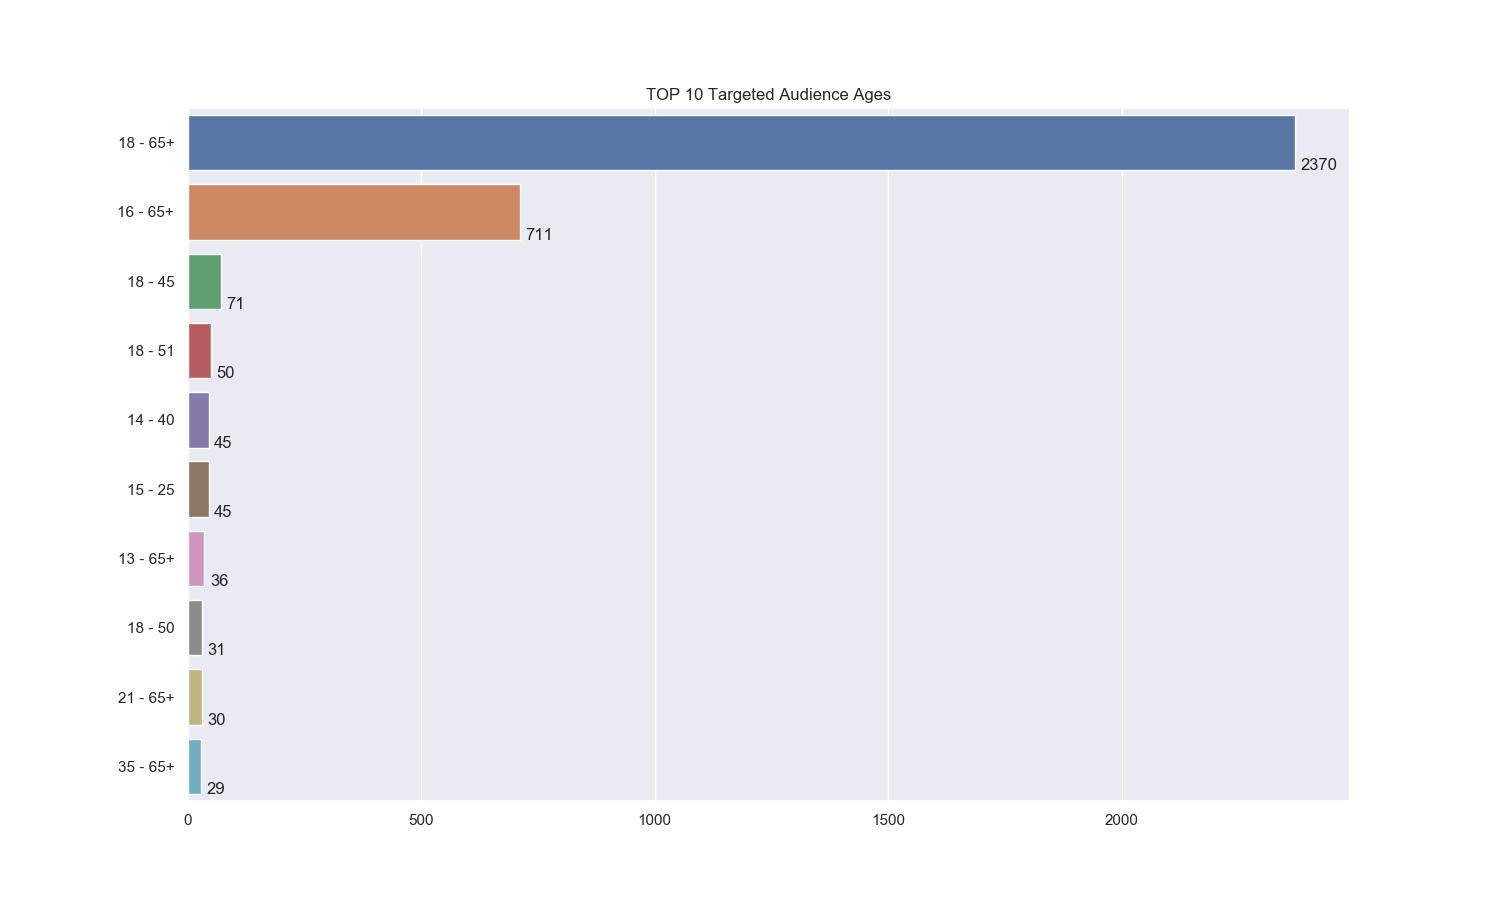
\includegraphics[width=\columnwidth]{./image/barchart-plots/barchart_targeted_age.png}
\caption{Distribution of Posts Based on Age (Years 2015, 2016, and 2017).}
\end{figure}

Interestingly, nearly all advertisements which targeted the age category of
15 -- 25 were all featuring the website \url{musicfb.info} which
~\cite{musicfb-info} appears to be a Chrome extension (currently unavailable)
and was registered in Saint Petersburg, Russia (location of IRA headquarters).

%%%%%%%%%%%%%%%%%%%%%%%%%%%%%%%%%%%%%%%%%%%%%%%%%%%%%%%%%%%%%%%%%%%%%%%%%%%%%%%
% Regression Analysis
%%%%%%%%%%%%%%%%%%%%%%%%%%%%%%%%%%%%%%%%%%%%%%%%%%%%%%%%%%%%%%%%%%%%%%%%%%%%%%%

\section*{\centering Regression Analysis}
\addcontentsline{toc}{section}{Regression Analysis}

We would like to determine if there is a statistically significant relationship
between two quantitative variables: the textual length of advertisement and the
money paid for it. Determinining the relationship between these variables will
give us an idea if there was some kind of priority attached to posts, depending
on its textual length.

\bigskip

For this task, we use a linear regression approach. Note that we perform the
test only on the ads paid in rubles, the primary reason being not having enough
data points for USD (only 5 values).

\begin{figure}[H]
  \centering
  \subfloat[Money Spent VS Ad Spend Length]{{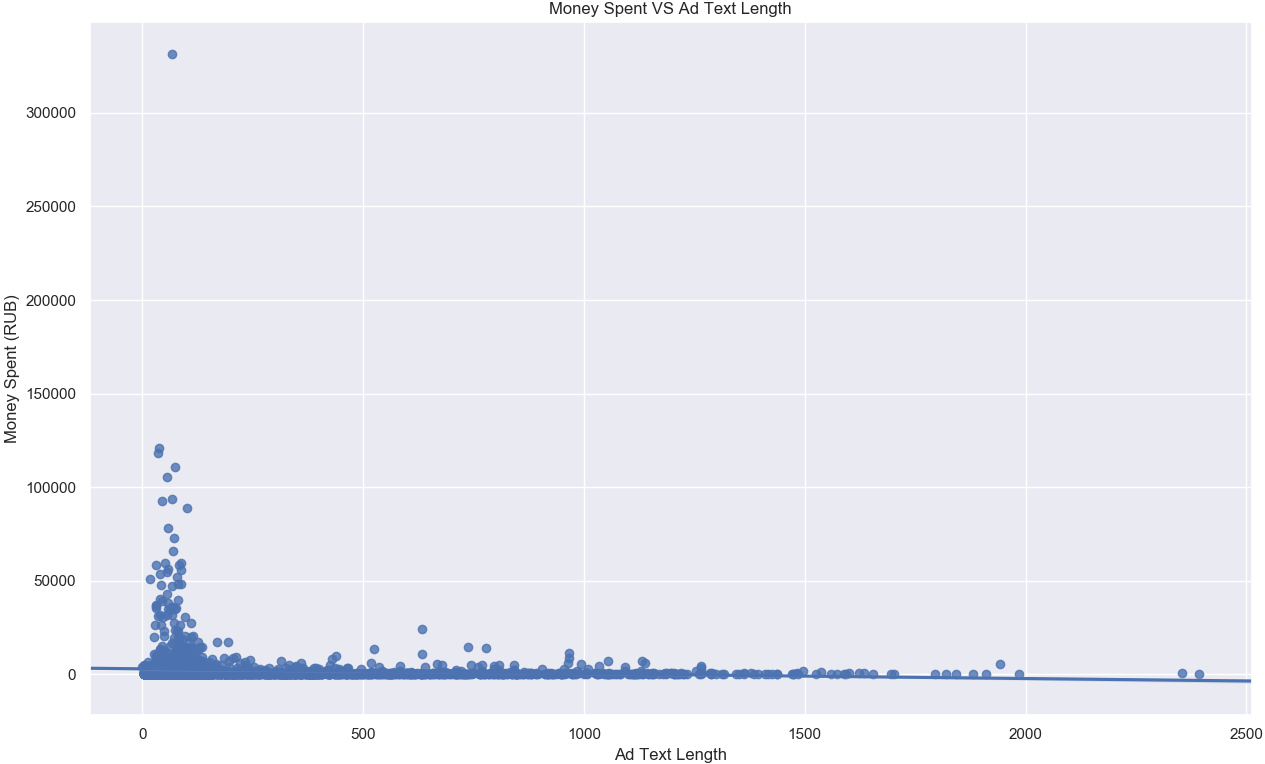
\includegraphics[width=8cm]{./image/regression-plots/ad_spend_text_length_regression.png}}}
  \hfill
  \subfloat[Log Money Spent VS Log Ad Spend Length]{{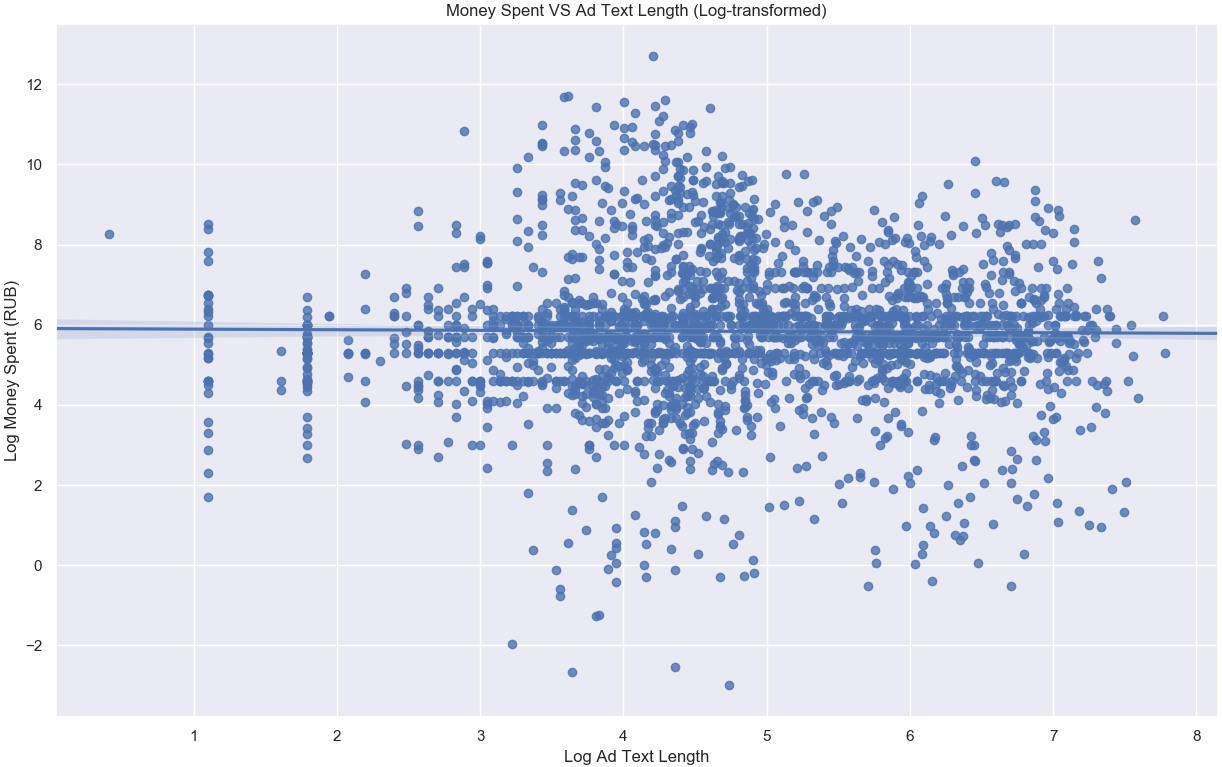
\includegraphics[width=8cm]{./image/regression-plots/ad_spend_text_length_regression_log_transform.png}}}
  \caption{Simple VS Log-transformed}
  \label{fig:example}
\end{figure}

\bigskip

The first plot showed no strong relationship between the response and the
predictor. That said, the shape of the plot hinted us to apply the log
transformation. The log transformation, once again, verified our assumption
of no relationship. The numerical data shown in Figure 9 further reinforces our
observations.

\bigskip

\begin{figure}[H]
\begin{center}
\begin{tabular}{|p{3cm}|p{3cm}|}
 \hline
 \multicolumn{2}{|c|}{RUB (Without Log Transform)}\\
 \hline
 Slope          & -2.594\\
 \hline
 Intercept      & 2980.780\\
 \hline
 R-squared      & 0.007\\
 \hline
 P-value        & $3.680 * 10^{-5}$\\
 \hline
 Standard Error & 0.627\\
 \hline
\end{tabular}
\qquad
\begin{tabular}{|p{3cm}|p{3cm}|}
 \hline
 \multicolumn{2}{|c|}{RUB (With Log Transform)}\\
 \hline
 Slope          & -0.015\\
 \hline
 Intercept      & 5.904\\
 \hline
 R-squared      & 0.0001\\
 \hline
 P-value        & $0.594 * 10^{-5}$\\
 \hline
 Standard Error & 0.028\\
 \hline
\end{tabular}
\end{center}
\caption{Linear Regression Analysis Results.}
\end{figure}

\bigskip

From the chart above, we see the R-squared value of \$0.007, which tells us
that only 0.7\% of variation in the money paid for advertisements is explained
by the number of words. Standard error is 0.627 which is very small compared
to the intercept whose value is 2980.780 (RUB). This tells us that the error
in our estimates is really small. The p-value equals $3.680 * 10^{-5}$ which
is a lot smaller than $0.05$ and makes the conclusion statistically significant.

\bigskip

Even after performing a log-transform, the results show no evidence of a strong
or even a weak relationship between the variables. The p-value tells us that
the results are statistically significant.

\bigskip

Although having no relationship is usually not a desired result, in our case,
we can conclude that posts were designed in a rather intelligent manner, with
no noticeable priorities depending on the number of words in the text section.

%%%%%%%%%%%%%%%%%%%%%%%%%%%%%%%%%%%%%%%%%%%%%%%%%%%%%%%%%%%%%%%%%%%%%%%%%%%%%%%
% Conclusions
%%%%%%%%%%%%%%%%%%%%%%%%%%%%%%%%%%%%%%%%%%%%%%%%%%%%%%%%%%%%%%%%%%%%%%%%%%%%%%%

\section*{\centering Conclusions}
\addcontentsline{toc}{section}{Conclusions}

We have scraped PDF files made publicly available by The United States House
Permanent Select Committee on Intelligence and performed a number of different
analyses including textual and statistical. The results obtained gave us
insights about the approaches used in the influence campaign. That said, there
is a lot more that could be analyzed using the provided datasets and any
researcher and/or interested person is free to use them for their own research.

%%%%%%%%%%%%%%%%%%%%%%%%%%%%%%%%%%%%%%%%%%%%%%%%%%%%%%%%%%%%%%%%%%%%%%%%%%%%%%%
% Bibliography and References
%%%%%%%%%%%%%%%%%%%%%%%%%%%%%%%%%%%%%%%%%%%%%%%%%%%%%%%%%%%%%%%%%%%%%%%%%%%%%%%

\newpage

\begin{center}
\printbibliography[heading=bibintoc]
\end{center}

%%%%%%%%%%%%%%%%%%%%%%%%%%%%%%%%%%%%%%%%%%%%%%%%%%%%%%%%%%%%%%%%%%%%%%%%%%%%%%%
% The end of the document
%%%%%%%%%%%%%%%%%%%%%%%%%%%%%%%%%%%%%%%%%%%%%%%%%%%%%%%%%%%%%%%%%%%%%%%%%%%%%%%

\end{document}
